% Emacs, this is -*-latex-*-

\label{sec:DBS}

\begin{notex}
  Finished and implemented.
\end{notex}

\acrshort{DBS} is the most basic set of rules. The rest of sets extends or modify
its functionality.

\begin{table}
  \centering
  \begin{tabular}{rl}
    Parameter & Meaning \\
    \hline
    $N^*$  & Maximum number of peers in a team \\
    $C$    & Chunk size \\
    $B$    & Buffer size, in chunks, in the peers \\
    $B'$   & Length of the list of the last $B'$ peers served by the splitter \\ 
    $D$    & Diameter of the flooding tree \\
    $L^*$  & Maximum allowed number of lost chunks \\
    $M$    & Number of monitors \\
    $R$    & Average bit-rate of the media \\
    Variable & \\
    \hline
    $N$    & Number of peers in the team \\
    $t_c$  & Chunk time \\
    $t_r$  & Round time \\
    $t_b$  & Buffering time \\
    $t_p$  & Physical network latency \\
    $t_s$  & Start-up time
  \end{tabular}
  \caption{Nomenclature used in DBS.} %
  \label{tab:DBS_nomenclature}
\end{table}

DBS provides \acrshort{ALM} of a \gls{media} \gls{stream} in an
\gls{unicast} environment. The media is sent by a streaming
\gls{server} (which is an external P2PSP entity), and received by a
\gls{splitter}\note{(see Sec.~\ref{sec:LBS})}~. The splitter divides
the stream into a sequence of \gls{chunk}s of data, and relay them to
a \gls{team} of peers, following a round-robing schema. Each peer of a
team gathers the chunks from the splitter and the rest of peers of the
team, and sends them to at least one \gls{player}\note{Peer should
  run even if no player(s) are connected to it.}~.

\begin{comment}
In single layered streams\footnote{Each layer of a
  scalable stream is received by a different peer attached to the same
  player capable or render scalable media.}, each peer is spawned by a
player (normal users should not run peers directly).
%This system has been described in Fig.~\ref{fig:DBS_system}.
\end{comment}

\begin{comment}
/* quitar: We define the set of teams as
$\{T\}$,
%=\{T^1,\cdots,T^{|T|}\}$,
and enumerate the peers in the team $T$ as $T=\{P_1,\cdots,P_{|T|}\}$. */
\end{comment}


\subsection{Feeding the team}
%%% Local Variables:
%%% mode: latex
%%% TeX-master: "<none>"
%%% End:

\label{sec:feeding_the_team}

The splitter divides the stream into chunks of constant length $C$
(see Tab.~\ref{tab:DBS_parameters}), and sends exclusively each
chunk to a different \emph{origin peer}\footnote{In the route that a
  chunk trances inside of the team, the origin peer of a chunk is
  first peer that receives that chunk, i.e. the peer selected by the
  splitter.}, using a round-robin schema. Chunks are enumerated to
distinguish them, and this information is transmitted as a part of a
chunk \emph{header}.

\begin{comment}
More details about the implementation
are available in Fig.~\ref{fig:chunk_generation}.

%$x$, conforming a message
%$c_x=[x,\text{chunk}]$, where
%$x=i \text{mod} \text{Splitter\_DBS.list\_of\_peers}.\text{length}()$.

\begin{figure*}
  %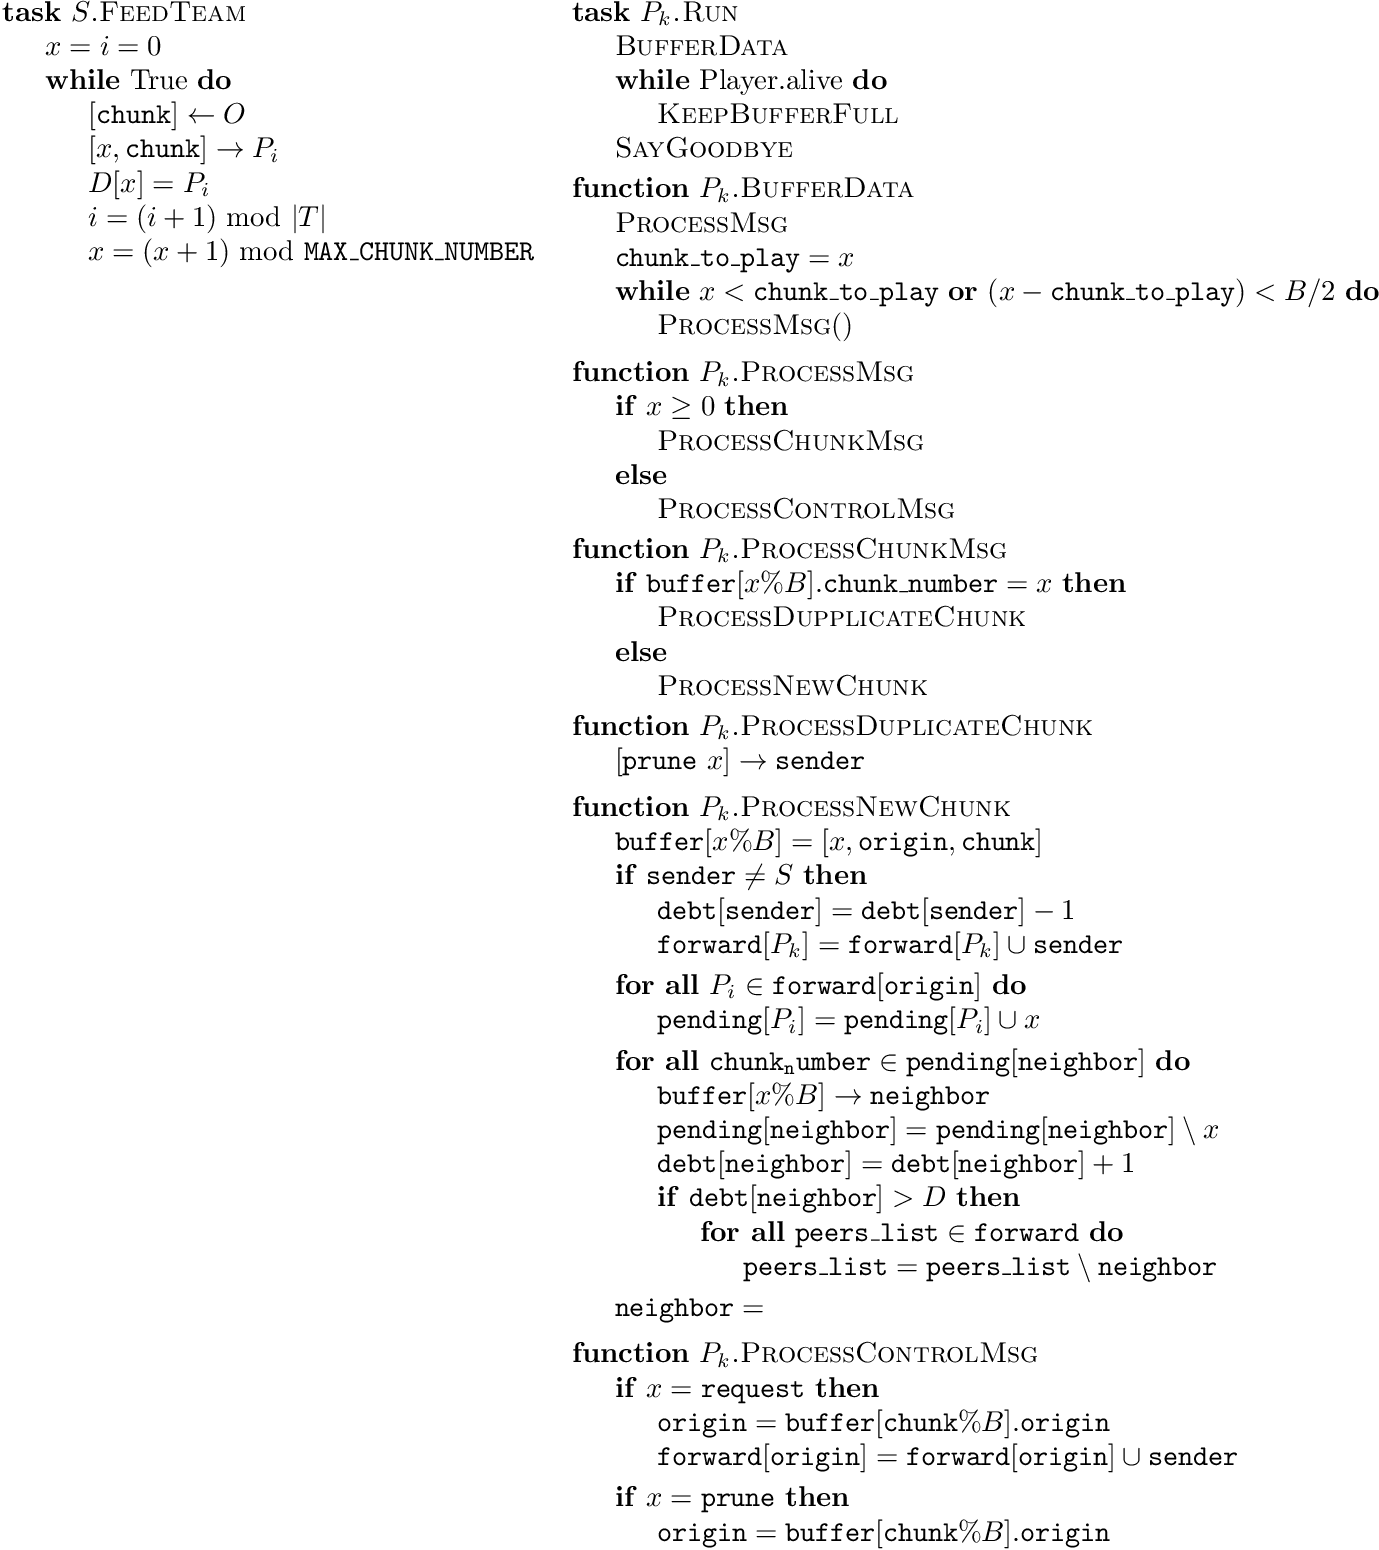
\includegraphics[width=0.75\textwidth]{chunk_generation_and_flooding}
  \fig{500}{5cm}{DBS_splitter_feed} \caption{Chunk
    generation at the splitter and their transmission to the
    team.\label{fig:chunk_generation}}
\end{figure*}
\end{comment}

We define a \emph{round} as the process of transmitting $N\leq N^*$
(see Tab.~\ref{tab:DBS_parameters}) different chunks from the splitter
to a team of $N$ peers. Therefore, for a team of size $N$, the
\emph{round-time} $t_R$ (see Tab.~\ref{tab:DBS_nomenclature}) is $N$
chunk-times. Notice that $t_R$ is generally variable, and depends on
the current number of peers in the team ($N$) and the chunk time
($t_C$) which depends on the chunk size ($C$, see
Tab.~\ref{tab:DBS_parameters}), and the average bit-rate of the media
stream.

The splitter remembers which chunk, of a list of the last $B'$ (see
Tab.~\ref{tab:DBS_parameters}) transmitted chunks, was sent to each
peer of the team. Notice that, in order to remember the chunk that was
sent to each peer in each round, must be hold that $B'\ge N$. \note{See
  \href{https://github.com/P2PSP/simulator/blob/f0c73be1817e7d3b816cc61cd2c8e59b17f9a0e6/src/core/splitter_dbs.py\#L296}{$\text{destination\_of\_chunk}[]$
    in \texttt{splitter\_dbs.py}}.}

\begin{comment}
(in a team) as the time necessary to send two consecutive chunks from
  the splitter (of such team) to the same peer, using the
  round-robing. This time is variable and depends on $|T|$, $C$, and
  the average bit-rate of the media, $A$.
\end{comment}

\begin{comment}
The round-time is defined by:
\begin{equation}
  \cal{r} = \cal{c}N.
  \label{eq:round_time}
\end{equation}
For example, if we use only one team of $N=256$ peers, a chunk size
$C=1024$~bytes, and a video of $1$~Mb/s, the round time is
\begin{displaymath}
  \cal{r} = \frac{1024\frac{\text{bytes}}{\text{chunk}}\times
    8\frac{\text{bits}}{\text{byte}}}{10^6\frac{\text{bits}}{\text{second}}}\times
  256 \approx 2.1~\text{seconds}.
\end{displaymath}
\end{comment}


\subsection{Joining a team}
% Emacs, this is -*-latex-*-

% Joining the Team

\label{sec:joining}

After connecting with a splitter\footnote{A team can be fed by more
  than one splitter in order to introduce redundancy in single-layer
  stream to deal with the loss of chunks, or when using MDC each
  stream description is transmitted by a different splitter.},
incoming peers request (using a reliable communication) to the
splitter the current list of peers in the team $T$. To minimize the
\gls{joining-time}, the peer sends a $[\mathtt{hello}]$ message to
each other peer of the team, in parallel with the reception of the
list. When a peer of the team receives a $[\mathtt{hello}]$, it adds
the sender of the message to the team list\footnote{Peers also updates
  their team list every time a chunk is received from a peer,
  incorporating the sender and the origin of the chunk.} and to a
jagged array of peers called $\mathtt{f}[]$ \note{(see
  \href{https://github.com/P2PSP/simulator/blob/f0c73be1817e7d3b816cc61cd2c8e59b17f9a0e6/src/core/peer_dbs.py\#L491}{$\text{f[]}$
    in \texttt{peer.py}})}. If a peer $P_i$ has an entry
$\mathtt{f}[P_j]=\{P_k\}$, then each chunk received by $P_i$ and
originated at $P_j$ will be forwarded to $P_k$. When an incoming peer
$P_i$ has received the list of peers, its forwarding table has been
initialized to $\mathtt{f}[P_i]=\{T\setminus P_i\}$. Notice that, as
long as the forwarding table contains this information, all the chunks
received from the splitter will be forwarded to the rest of the team,
directly (in one single hop/chunk). So, in absence of communication
constraints, the team will be organized as a full-connected overlay
(see Fig.~\ref{fig:three_topos}-(a)).

\begin{figure}
  \centering
  \myfig{graphics/topologies}{\columnwidth}{800}
  \caption{Different overlay (team) topologies.}
  \label{fig:three_topos}
\end{figure}%
  
%\begin{figure}%
%  \centering
%%  \subfigure[A full-connected overlay.]{%
%%    \label{fig:full}%
%%    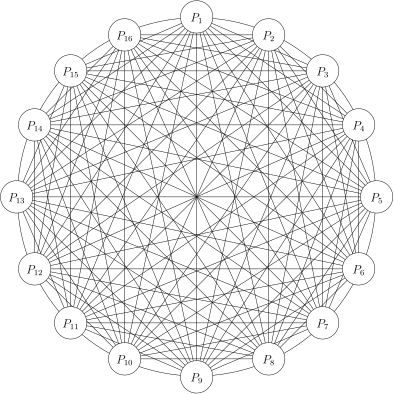
\includegraphics[width=0.45\textwidth]{graphics/full-mesh}}%
%%  \qquad
%%  \subfigure[A star-shaped overlay.]{%
%%    \label{fig:star}%
%%    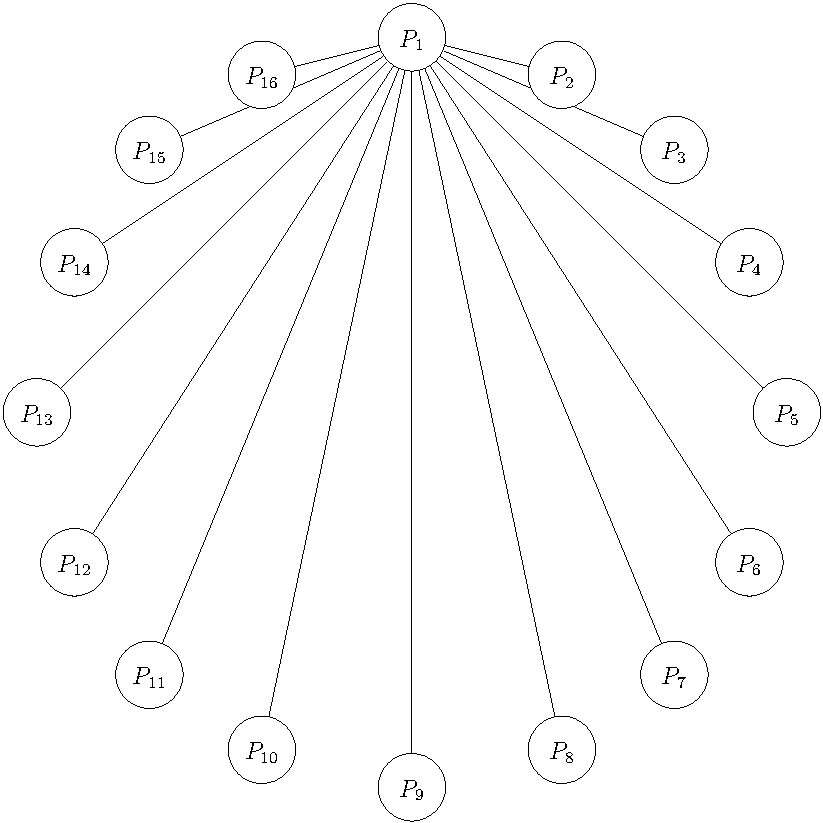
\includegraphics[width=0.45\textwidth]{graphics/star}}%
%\begin{tabular}{ccc}
%  %\subfigure[Full-connected. $\forall P_i\in T, \mathtt{f}[P_i]=T\setminus P_i$]{%
%  %\subfigure{Full-connected. \newline $\forall P_i\in T, \mathtt{f}$[$P_i$]}{%
%  \subfigure{Full-connected}{%
%    \label{fig:full}%
%    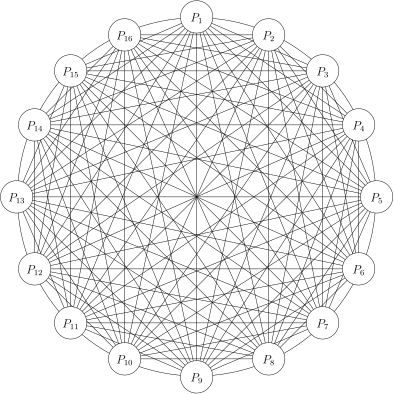
\includegraphics[width=0.3\textwidth]{graphics/full-mesh}}%
%  &
%  \subfigure[Star-shaped.]{%
%    \label{fig:star}%
%    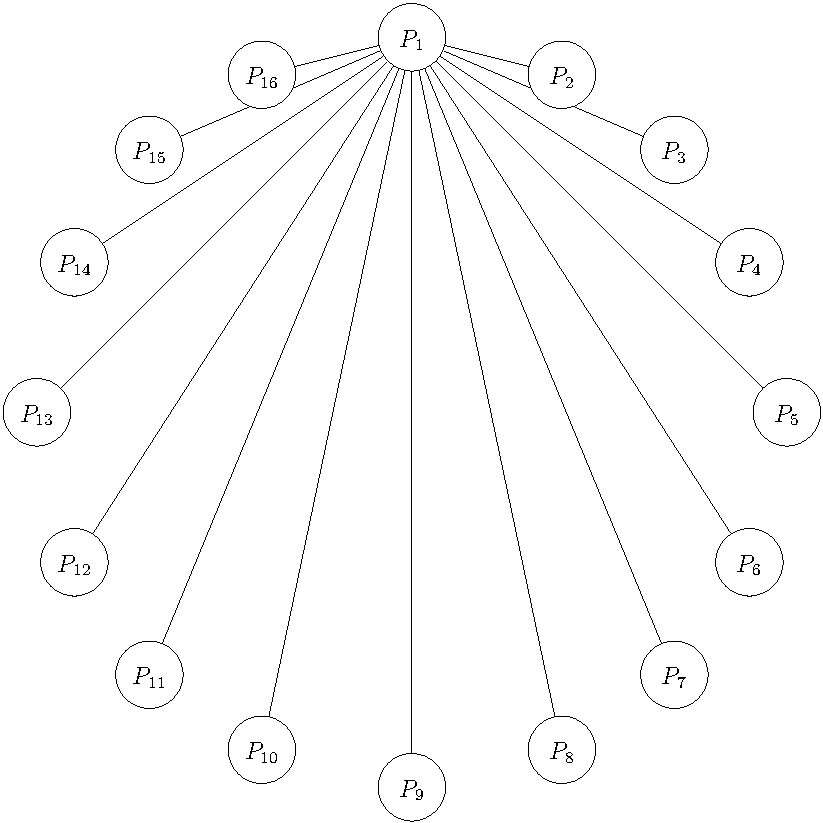
\includegraphics[width=0.3\textwidth]{graphics/star}}%
%  &
%  \subfigure[Ring-shaped.]{%
%    \label{fig:ring}%
%    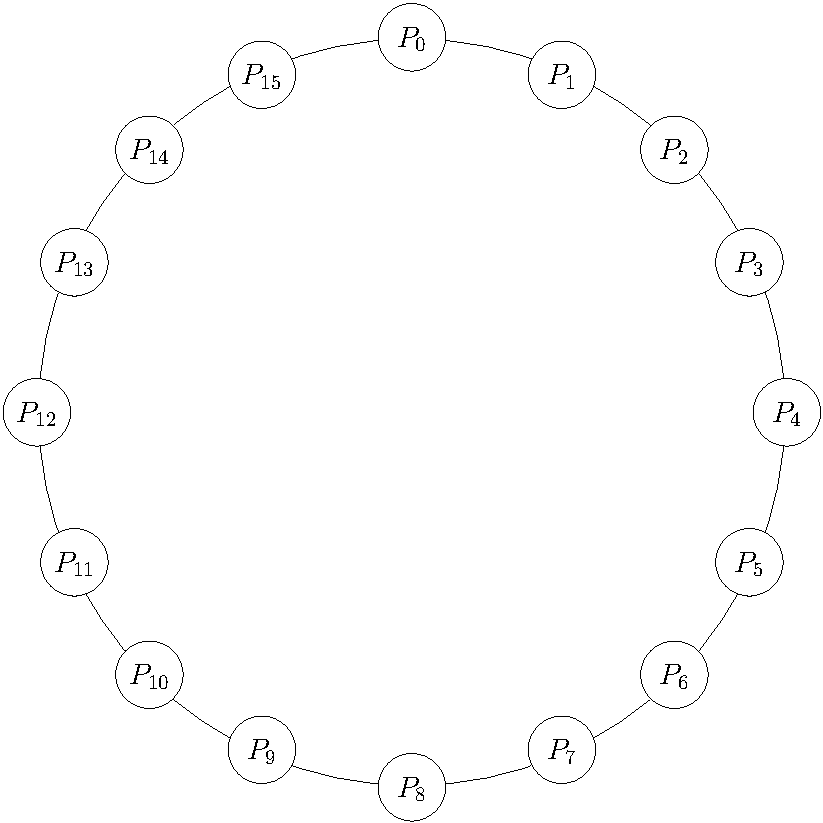
\includegraphics[width=0.3\textwidth]{graphics/ring}}%
%\end{tabular}
%  \caption{Different overlay (team) topologies.}
%  \label{fig:connections}
%\end{figure}

%), initializes
%the table $\mathrm{debt}[]$ (which stores the chunk debts between
%neighbor peers), and (3) sets the variable $\mathrm{neighbor}$ with an
%index to $\mathrm{f}[]$ (see
%Sec.~\ref{sec:chunk_DBS_processing}).

The splitter, in an infinite loop: (1) listens to the incoming peers,
(2) sends to them the list of peers of the team, (3) includes the
incoming peer to the list, and (4) send a copy of the stream to the
team using a round-robing, as a sequence of chunks. Notice that only
those peers that are in the list of peers of the splitter are
considered to be in the team served by such splitter.

\begin{comment}
\begin{figure*}
  %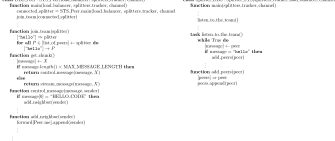
\includegraphics[width=\textwidth]{joining}
  \fig{1000}{10cm}{joining} \caption{Code related to team
    joining.\label{fig:joining}}
\end{figure*}

The new pseudo-code related to joining a team is describen in the
Fig.~\ref{fig:joining}.
\end{comment}

\begin{notex}
  See \href{https://github.com/P2PSP/simulator/blob/f0c73be1817e7d3b816cc61cd2c8e59b17f9a0e6/src/core/splitter_dbs.py#L296}{$\text{destination\_of\_chunk}[]$ in \texttt{peer\_dbs.py}}.
\end{notex}


\subsection{Chunk flooding}
%%% Local Variables:
%%% mode: latex
%%% TeX-master: "<none>"
%%% End:

\label{sec:chunk_flooding}

\begin{comment}
\begin{figure*}
  %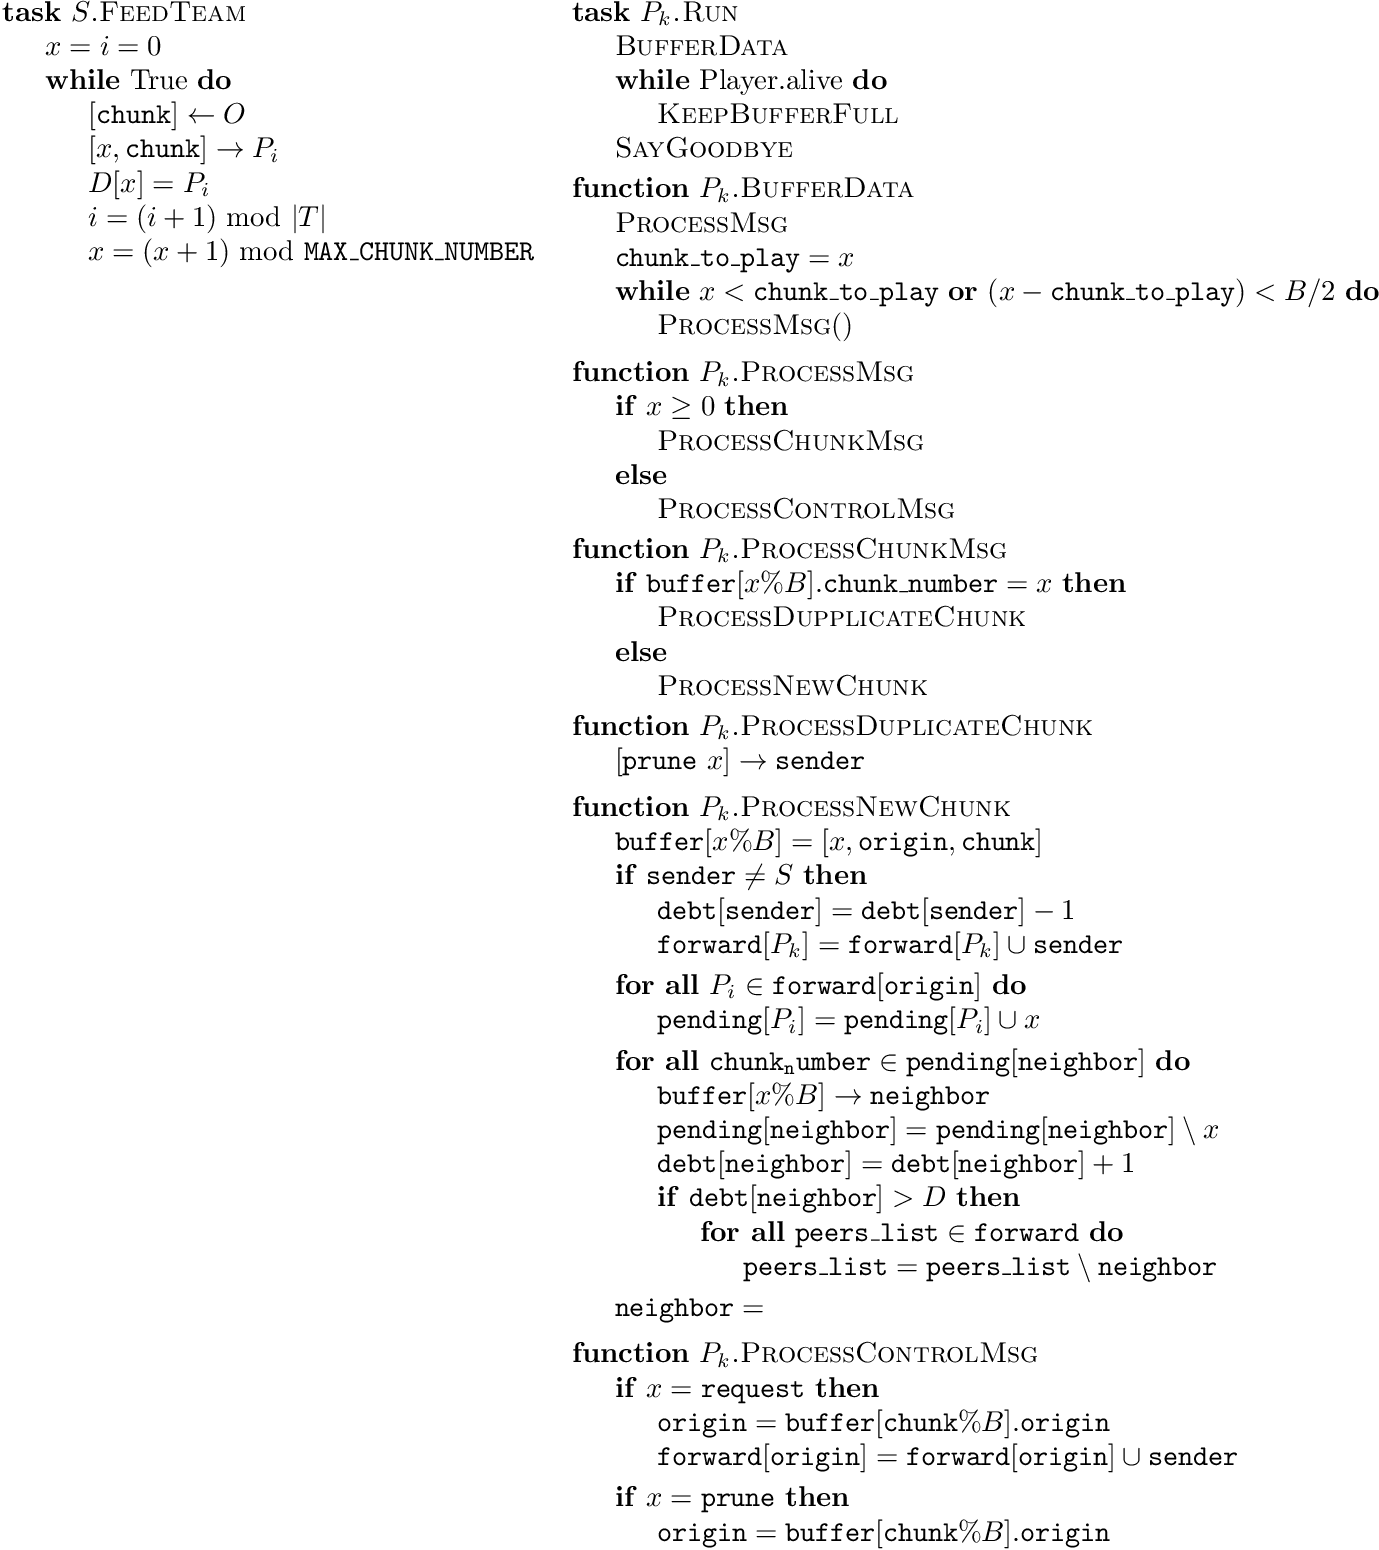
\includegraphics[width=0.75\textwidth]{chunk_generation_and_flooding}
  \imgw{300}{graphics/peer_chunk_flooding.svg}
  \caption{Chunk flooding at peers.\label{fig:peer_chunk_flooding}}
\end{figure*}
\end{comment}

DBS implements a push-based protocol. When a peer receives a chunk, it
can be retransmitted to a large number of neighbors (depending on the
number of different destinations in its forwarding table). Therefore,
even by controlling the chunk rate in the servers\footnote{Using DBS
  the data-flow can not be controlled in the peers or the splitter
  because they don't understand the stream.}, some kind of flow
control must be performed in order to reduce network congestion while
peers perform the flooding.

%Moreover, to achieve an ideal I/O ratio of $1$, peers should send one
%chunk for every received one.

\begin{figure*}
  \centering
  \subfloat[A full-connected overlay.]{\label{fig:full_mesh}
    \vbox{\myfig{graphics/full-mesh}{6cm}{250}}}
  \quad
  \subfloat[A star-shaped overlay.]{\label{fig:star}
    \vbox{\myfig{graphics/star}{6cm}{250}}}
  \caption{In a full-connected DBS team (see Subfig. (a)), all peers
    receive and send the same number of chunks. In a star-shaped DBS
    team such as the shown in the Subfig. (b), $P_1$ should send all
    the chunks of the stream to the rest of the team, except those
    that the splitter has sent directly to the rest of peers.}
\end{figure*}

The congestion (in particular, the one caused by how DBS nodes use the
physical links) may be avoided by means of a basic idea: \textit{if I
have received a chunk, I should send a chunk (not necessary to the
sender)}. It is easy to see that, in a fully connected overlay
(Fig.~\ref{fig:full_mesh}), this allows to control the data
flow. However, in more realistic scenarios (such as those in which
firewalls and symmetric NATS are used), where the physical media
imposes interconnexion constraints, peers can not be ``connected''
with the rest the team, and therefore, if the splitter follows a pure
round-robin strategy, some peers can send more chunks that they
receive (see the Fig.~\ref{fig:star}). In these scenarios, the simple
rule of sending a chunk for each received one does not work.

The previous idea can be adapted to handle a variable connectivity
degree (also called \emph{neighborhood degree}) if each peer uses a
table of lists, $\mathtt{pending}{}$, indexed by the neighbor's
end-points, where each list stores the positions in the buffer of
those chunks that must be transmited to the corresponding neighbor,
the next time such neighbor be selected in the flooding process. Thus,
for example, if $\mathtt{pending}\{P_x\}=\{11,22\}$, chunks found at
positions $11$ and $22$ of the buffer have to be sent to peer $P_x$
(when the pending scheduler used by the peer selects $P_x$).

Notice that using this procedure, more than one chunk can be sent to a
neighbor in a transmission burst, which could congest the switching
devices. However, except in very unbalanced overlays
(Fig.~\ref{fig:star}), the bursts use to be very short (only one chunk
in most of cases). As an advantage, if a burst is produced, all the
chunks of the burst travel between the two same hosts, which usually
increases the performance of the physical routing.

An example of the temporal evolution of a team using this behaviour
has been described in the Figures \ref{fig:team_0}, \ref{fig:team_1}
and \ref{fig:team_2}.

\begin{figure}
  \myfig{graphics/team_0}{4cm}{250} %
  \caption{A team has been created with a single monitor $M_0$
    ($[\mathtt{hello}]$ messages are not shown). Chunks with indexes 0
    and 1 (the time $t$ is measured in chunks-time) have been
    transmitted from the splitter $S$ to $M_0$. $f$ and $p$ represents
    the $\text{forward}[]$ and the $\text{pending}[]$ structures,
    respectively. The chunks stored in the buffer are shown below the
    entity.} %
  \label{fig:team_0}
\end{figure}

\begin{figure}
  \myfig{graphics/team_1}{4cm}{250} %
  \caption{At $t_2$, peer $P_1$ joins the team (the
    $[\mathtt{hello}]$'s are not shown). In $M_0$, $f=\{M_0:[P_1]\}$
    because when $M_0$ receives the $[\mathtt{hello}]$ from $P_1$,
    $M_0$ is the origin peer for all chunks received from $S$ and
    $P_1$ is its neighbor. $P_1$ includes an entry $P_1:[M_0]$ in its
    forwarding table because $M_0$ is in the list of peers received
    from the splitter. After that, when the chunk number 2 arrives to
    $M_0$ from $S$, an entry $P_1:2$ is created in $P\{\}$ for that
    chunk, and this entry is deleted when the chunk 2 is sent to
    $P_1$.} %
  \label{fig:team_1}
\end{figure}

\begin{figure}
  \myfig{graphics/team_2}{4cm}{300} %
  \caption{$P_2$ joins the team. $M_0$ and $P_1$ includes $P_2$ in
    their forwarding tables. The chunk 3 is received by $P_1$ which
    decides to send it to $P_2$. Chunk 3 remains as pending to be sent
    to $M_0$ when the next chunk is received by
    $P_1$.} %
  \label{fig:team_2}
\end{figure}
%  $P_2$ is the origin peer for $M_0$ and $P_1$ because both of them are in the list of peers that $P_2$ receives from $S$.
    
\begin{figure}
  \myfig{graphics/team_3}{4.5cm}{330} %
  \caption{Chunk 4 is received by $P_2$ which relays it to $P_1$, what
    relays chunk 3 to $M_0$.} %
  \label{fig:team_3}
\end{figure}

\begin{figure}
  \myfig{graphics/team_4}{4.5cm}{330} %
  \caption{Chunk 5 is received by $M_0$ which
    relays it to $P_2$.} %
  \label{fig:team_4}
\end{figure}

\begin{notex}
  \begin{figure*}
    \myfig{graphics/team_5}{4cm}{350}
  \end{figure*}
  
  \begin{figure*}
    \myfig{graphics/team_6}{4cm}{380}
  \end{figure*}
  
  \begin{figure*}
    \myfig{graphics/team_7}{4cm}{320}
  \end{figure*}
  
  \begin{figure*}
    \myfig{graphics/team_8}{4cm}{200}
  \end{figure*}
  
  \begin{figure*}
    \myfig{graphics/team_9}{4cm}{280}
  \end{figure*}
  
  \begin{figure*}
    \myfig{graphics/team_10}{4cm}{380}
  \end{figure*}
  
  \begin{figure*}
    \myfig{graphics/team_11}{4cm}{210}
  \end{figure*}
  
  \begin{figure*}
    \myfig{graphics/team_12}{4cm}{210}
  \end{figure*}
  
  \begin{figure*}
    \myfig{graphics/team_13}{4cm}{210}
  \end{figure*}

\end{notex}

%An example of the flooding with congestion control algorithm has been
%show in the Figs.~\ref{fig:team_0}, ...
%Notice that in this example
%all messages are received successfully.
%As can be seen in the example, when a peer $P_k$ receives a chunk,
%$P_k$ floods a number of chunks to one of its its neighbors (obviously,
%except the neighbor sender of the chunk), using round-robin
%schema. The size of this set, what we call $\text{pending}$, depends
%on how many neighbors a peer has.

% Alternative: increment by +1 and decrement by /2

% Alternative: peers keep sorted the neighbors by debt, and the list
% is run from the beginning each time a chunk arrives from the
% splitter.

% Alternative: the debt is only incremented if the relayed chunk has
% been received from the splitter.

% Alternative: if between two consecutive chunks received from the
% splitter (a round), a peer does not receive a chunk from a neighbor
% with origin such neighbor, the peer is removed from the forwaring
% list.

\begin{comment}
In each round, peers check if a chunk have been received from the rest
of peers of the team (${\cal P}_k\in {\cal T}_j)$). If not, peers send
a $[\mathtt{propagate}~{\cal P}_i]$ to one or more (possibly
to the rest of) peers of the team, where ${\cal P}_i$ is the origin peer
of the missing chunk. At this point, the process continues as
described in Section~\ref{dbs:chunk_flooding}.
\end{comment}

\begin{comment}
For each ${\cal P}_k\in N({\cal P}_i)$, ${\cal P}_i$ checks if a chunk
has been received from ${\cal P}_k$. If ${\cal P}_i$ detects that
${\cal P}_k$ has not sent a chunk to it during $L$ consecutive rounds,
performs $N({\cal P}_i) = N({\cal P}_i)\setminus{\cal P}_k$, and stops
sending to ${\cal P}_k$ more chunks.
\end{comment}
\begin{comment}
computes a
``chunk-debt'', denoted by $d({\cal P}_k)$, that is incremented each
time a chunk is received from ${\cal P}_k$ and decremented each time a
chunk is sent to ${\cal P}_k$. If ${\cal P}_i$ verifies that $d({\cal
  P}_k)>D$ (the maximum debt), then ${\cal P}_i$ considers that ${\cal
  P}_k$ is unable to communicate with it, performs $N({\cal P}_i) =
N({\cal P}_i)\setminus{\cal P}_k$, and stops sending to ${\cal P}_k$
more chunks.
\end{comment}

%When peers receive chunks from their splitter, they must flood them to
%their neighbors until the chunks are broadcasted to the whole team
%(Fig.~\ref{fig:chunk_generation_and_flooding}). Lets suppose that
%${\cal P}_k$ receives a chunk. In the case the sender is its splitter,
%${\cal P}_k$ floods the chunk to $N({\cal P}_k)$. However, if the
%sender is a peer ${\cal P}_m\in N({\cal P}_k)$, ${\cal P}_k$ adds
%${\cal P}_m$ to $N({\cal P}_k)$ if ${\cal P}_m$ is a new neighbor, and
%forwards the chunk to the rest of its neighborhood ${\cal P}_n\in
%N({\cal P}_k)\setminus{\cal P}_m$ if ${\cal P}_k$ is in the shortest
%between ${\cal P}_n$ and the origin peer ${\cal P}_i$ of the relayed
%chunk. This will be true if ${\cal P}_k$ is the gateway of ${\cal
%  P}_n$ to go from ${\cal P}_n$ to ${\cal P}_i$. Therefore, a flooding
%with prunning based on shortest path routing is used.

%Peers do not understand the content, but it is
%known that in order to achieve a I/O ratio of 1, peers should send one
%chunk for every received one, on average. To acomplish this, a ${\cal
%  P}_i$ creates a FIFO queue of chunks for each $N({\cal P}_i)$, and,
%for each received chunk, ${\cal P}_i$ forwards a queued chunk from
%each of these queues.

\begin{comment}
A ${\cal P}_i$ forwards one or more chunks if and only if it has
received a chunk. For each received chunk $c_j$, ${\cal P}_i$: 1)
creates a list $l_{c_j}$ with the contents of $N'({\cal P}_i)$, and 2)
sends $c_j$ to $l_{c_j}[0]$ (the first element), and removes
$l_{c_j}[0]$. For each chunk reception, Step 2) is repeated for all
the previously created lists while they are not exhausted.

A solution is a forwarding algorithm based on the following
idea. Peers manage a list of chunks, where every item is a 2-tuple
($c_k$, $P_l$). The field $c_k$ represents the chunk that must be
flooded (if the node that has delivered the chunk is the splitter,
$c_k$ must be relayed towards all the neighbors, otherwise, $c_k$ must
be sent to all the neighbors except the peer that delivered $c_k$),
and the field $P_l$ the last neighbor to which $c_k$ was sent. For
every chunk received, a new tuple is appended to the list of chunks
and the rest of tuples are updated. The field $c_k$ remains constant
but $P_l$ is replaced by the next peer in the list of neighbors for
every received chunk.
\end{comment}


\subsection{Buffering chunks}
% Emacs, this is -*-latex-*-

% Buffering chunks

\label{sec:buffering_chunks}

In order to hide the jitter generated by the physical network and the
protocol itself, peers need to store the received chunks in a buffer
during a period of time, before sending them to a player. A chunk with
number $x$ is inserted in the position $(x~\mathit{mod}~2B)$ of the
buffer, where $B$ is the maximum number of chunks that the buffer
stores. In a peer's life, $B$ is a constant specified by the user,
but it is not compulsory that all peers of a team use the same buffer
size.

The buffer is implemented as a circular queue of $2B$ chunks, what is
filled with up to $B$ chunks during the \gls{buffering-time} $t_b$,
which is the main part of the \gls{start-up-time} experienced by
users. Chunks with a higher number (newer chunks) are inserted near of
(depending on the order in which the chunks arrive to the peer) the
head of the buffer. The (received) chunks pointed by the tail of the
buffer $p_p$ (the playing pointer) are sent to the player. This action
is carried out each time a new chunk is received\footnote{DBS does not
  know anything about the content and therefore, about the timing of
  the chunks.}. During the playing process, empty cells in the buffer
(caused by the chunks that have not been received on time) are skipped.

% Hablar de la relación entre B y el tamaño del team. Tal vez, cuando
% se presente la expresión de la latencia en función del grado de
% conectividad. En el caso extremo en que todos los peers se
% conectaran con todos, B >= N^*, el número máximo de peer en el team.


\subsection{Leaving a team}
\label{sec:leaving}

An outgoing peer must to: (1) say $[\mathtt{goodbye}]$ to the splitter
and the neighbor peers (in this order), (2) relay any pending
(received but yet not sent) chunks, and (3) wait for a
$[\mathtt{goodbye}]$ from the splitter, in this order. In case of
timeout, the leaving procedure is reset.

When a peer of the team receives a $[\mathtt{goodbye}]$, removes the
sender from the $\text{forward}$.

The splitter removes the peer from the list of peers.

\begin{figure*}
  %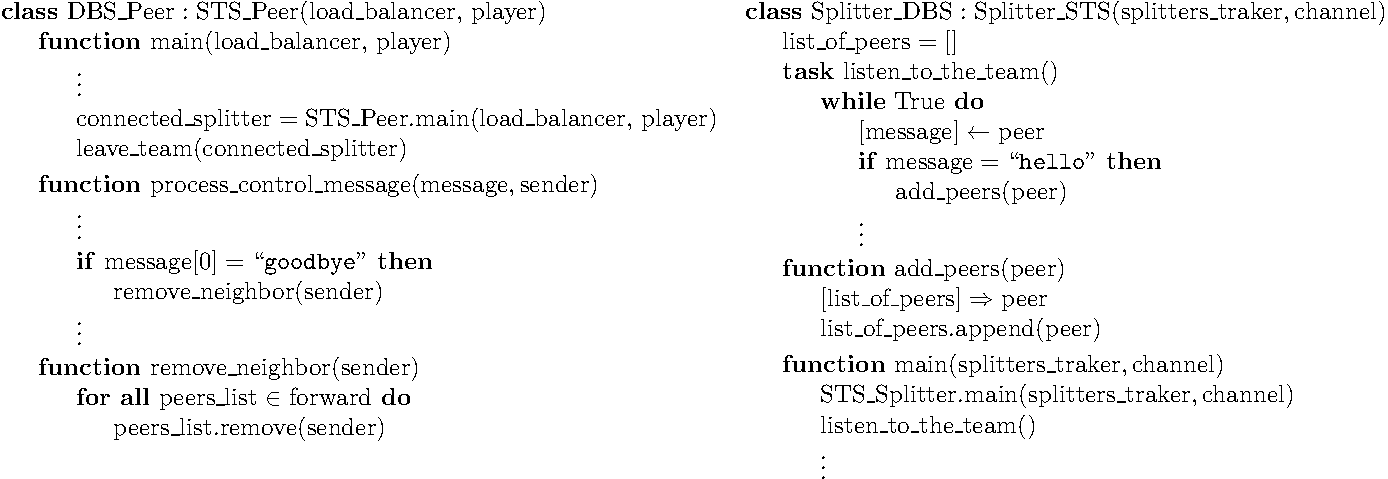
\includegraphics[width=0.55\textwidth]{leaving}
  \fig{400}{4cm}{leaving}
  \caption{Leaving a team.\label{fig:leaving}}
\end{figure*}

All these rules have been describen in Fig.~\ref{fig:leaving}.

\begin{comment}
An outgoing peer $P_o$ (see Fig.~\ref{fig:leaving}) must to: (1) say
$[\mathtt{goodbye}]$ to $S$ and to $T^o$ (in this order), (2)
relay any pending (received but yet not sent) chunks, and (3) wait for
a $[\mathtt{goodbye}]$ from $S$, which performs $T = T \setminus
P_o$. In case of a timeout, $P_o$ resets the leaving procedure,
for a maximum number of times.

When a $P_k$ receives a $[\mathtt{goodbye}]$ from $P_o$, $P_k$
removes $P_o$ from its neighbors set, by running $T^k = T^k
\setminus P_o$.
\end{comment}


\subsection{Free-riding control at splitters}
% Emacs, this is -*-latex-*-

% Free-riding Control at the Splitter

\label{sec:free_riding_control}

The splitter remembers which chunk, of a list of the last $B'$
transmitted chunks, was sent to each peer of the team. Notice that, in
order to remember the chunk that was sent to each peer in each round,
must be hold that $B'\ge N$. \note{See
  \href{https://github.com/P2PSP/simulator/blob/f0c73be1817e7d3b816cc61cd2c8e59b17f9a0e6/src/core/splitter_dbs.py\#L296}{$\text{destination\_of\_chunk}[]$
    in \texttt{splitter\_dbs.py}}.}

Monitor peers (which are trusted peers) complain to their splitter
with a $[\mathtt{lost}~\text{lost\_chunk\_number}]$ for each lost
chunk. The splitter only considers these type of messages if they come
from a monitor.

%Notice that $L$ will
%tend to be proportional to the number $M$ of monitors, especially if
%those cases where $P_o$ is a gone peer that was unable to transmit the
%$[\mathtt{goodbye}]$ messages.

\begin{notex}
This last functionality has not been implemented, at least, as it has
been explained here. The forget() thread is controlled by a timer, not
by a counter of rounds.
\end{notex}

%Peers also control that at least one chunk is received from a neighbor
%in each round.\footnote{Peers recognize that a new round has started
%  when a new chunk is received from the splitter.} If happens that a
%peer $P_x$ does not receives a chunk from peer $P_y$ between $D^*$
%consecutive rounds, $P_x$ removes $P_y$ of its forwaring table.


%\subsection{Free-riding control at peers} % Neighborhood dynamics
%\label{dbs:frcp}
%In each round, peers check if a chunk have been received from the rest
of peers of the team (${\cal P}_k\in {\cal T}_j)$). If not, peers send
a $[\mathtt{propagate}~{\cal P}_i]$ to one or more (possibly
to the rest of) peers of the team, where ${\cal P}_i$ is the origin peer
of the missing chunk. At this point, the process continues as
described in Section~\ref{dbs:chunk_flooding}.

\begin{comment}
For each ${\cal P}_k\in N({\cal P}_i)$, ${\cal P}_i$ checks if a chunk
has been received from ${\cal P}_k$. If ${\cal P}_i$ detects that
${\cal P}_k$ has not sent a chunk to it during $L$ consecutive rounds,
performs $N({\cal P}_i) = N({\cal P}_i)\setminus{\cal P}_k$, and stops
sending to ${\cal P}_k$ more chunks.
\end{comment}
\begin{comment}
computes a
``chunk-debt'', denoted by $d({\cal P}_k)$, that is incremented each
time a chunk is received from ${\cal P}_k$ and decremented each time a
chunk is sent to ${\cal P}_k$. If ${\cal P}_i$ verifies that $d({\cal
  P}_k)>D$ (the maximum debt), then ${\cal P}_i$ considers that ${\cal
  P}_k$ is unable to communicate with it, performs $N({\cal P}_i) =
N({\cal P}_i)\setminus{\cal P}_k$, and stops sending to ${\cal P}_k$
more chunks.
\end{comment}


%\subsection{Congestion control}
%\label{dbs:congestion_control}
%%%% Local Variables:
%%% mode: latex
%%% TeX-master: "<none>"
%%% End:

\label{sec:congestion_control}

DBS is a content-unaware push-based protocol, where when a peer
received a chunk, it can be retransmitted to a large number of
neighbors. To avoid network congestion while flooding, sending peers
must perform some kind of data flow-control.

%Moreover, to achieve an ideal I/O ratio of $1$, peers should send one
%chunk for every received one.

Congestion control is performed by means of the basic idea of, {\sl if
  I have received a chunk, I should send a chunk}. It is easy to see
that, in a fully connected overlay, this allows to control the data
flow. However, peers can be ``connected'' with a variable number of
neighbors and therefore, if the splitter follows a pure round-robin
strategy, some peers can send more chunks that they receive.

The previous idea can be improved to handle a variable connectivity
degree. Each peer use an array of FIFO queues, $\text{pending}[]$,
indexed by the neighbor end-points, where each queue stores buffer
positions. Thus, if for example $\text{pending}[P_x]=\{11,22\}$,
chunks found at positions $11$ and $22$ of the buffer have to be sent
to peer $P_x$ when the priority round-robin scheduler used by the peer
select $P_x$ (see Sec.~\ref{sec:chunk_flooding}).


............

in DBS is very simple: if a new chunk is
received, peers forward (using the flooding with prunning algorithm
described in Sec~\ref{dbs:chunk_generation_and_flooding}) each
received chunk to the next peer of their list of peers (following a
round-robin pattern).

%Peers do not understand the content, but it is
%known that in order to achieve a I/O ratio of 1, peers should send one
%chunk for every received one, on average. To acomplish this, a ${\cal
%  P}_i$ creates a FIFO queue of chunks for each $N({\cal P}_i)$, and,
%for each received chunk, ${\cal P}_i$ forwards a queued chunk from
%each of these queues.

\begin{comment}
A ${\cal P}_i$ forwards one or more chunks if and only if it has
received a chunk. For each received chunk $c_j$, ${\cal P}_i$: 1)
creates a list $l_{c_j}$ with the contents of $N'({\cal P}_i)$, and 2)
sends $c_j$ to $l_{c_j}[0]$ (the first element), and removes
$l_{c_j}[0]$. For each chunk reception, Step 2) is repeated for all
the previously created lists while they are not exhausted.

A solution is a forwarding algorithm based on the following
idea. Peers manage a list of chunks, where every item is a 2-tuple
($c_k$, $P_l$). The field $c_k$ represents the chunk that must be
flooded (if the node that has delivered the chunk is the splitter,
$c_k$ must be relayed towards all the neighbors, otherwise, $c_k$ must
be sent to all the neighbors except the peer that delivered $c_k$),
and the field $P_l$ the last neighbor to which $c_k$ was sent. For
every chunk received, a new tuple is appended to the list of chunks
and the rest of tuples are updated. The field $c_k$ remains constant
but $P_l$ is replaced by the next peer in the list of neighbors for
every received chunk.
\end{comment}


\begin{comment}
\subsubsection{Flooding order}
\label{dbs:flooding_order}
As an incentive mechanism~\cite{xu2006analysis}, peers relay received
chunks first to those peers that 
\end{comment}

%neighbors with lower chunk-debts.

\begin{comment}
\subsubsection{Team dynamics}
\label{dbs:team_dynamics}
${\cal P}_i$ adds to $N({\cal P}_i)$ those ${\cal P}_j$ that has sent
to ${\cal P}_i$ a chunk. If $N({\cal P}_i)>K$, periodically, ${\cal
  P}_i$ removes from $N({\cal P}_i)$ the peer with highest chunk-debt
and try to find in ${\cal T}_j\setminus N({\cal P}_i)$ a new peer using
$[\mathtt{hello}]$ messages.
\end{comment}

\begin{comment}
Peers use a buffer $b$ of chunks to hide the jitter generated by the
physical network and the broadcasting protocol. When a peer receives
$C_i$, it performs
\begin{equation}
  b[i~\text{mod}~B] = c_i,
\end{equation}
where ``mod'' represents the modulo operator and $B$ the buffer size
(in chunks). Basically, the buffer represents a sliding window that
moves over the stream synchronizely with the playing because the the
player consumes the chunks at the same chunk-rate the source produces
them.
\end{comment}

%%%%%%%%%%

\begin{comment}

\begin{itemize}

\item In the P2PSP, only monitor peers complains about lost
  chunks. This means that if a chunk that has been retransmitted by a
  peer is lost, it will be only retransmitted to all the peers of the
  team if the destination is a monitor peer and there is a unique
  monitor peer in the team. On the other hand, if the lost chunk was
  traveling from the splitter to a peer, all monitor peers will
  complain and this chunk will be retransmitted to the complete
  team. Therefore, only massively loss chunks will be retransmitted in
  the P2PSP. However, notice that a isolated missing chunk will
  produce negligible artifacts in the playback of one peer. In the
  Chain model, the lost of a chunk is handled between neighbour peers
  which means that all lost blocks should be, a priori, recovered.

\end{itemize}

%}}}

\end{comment}



\begin{comment}
\subsubsection{Shortest path computation}
\label{dbs:chunk_routing}
\begin{figure}
  %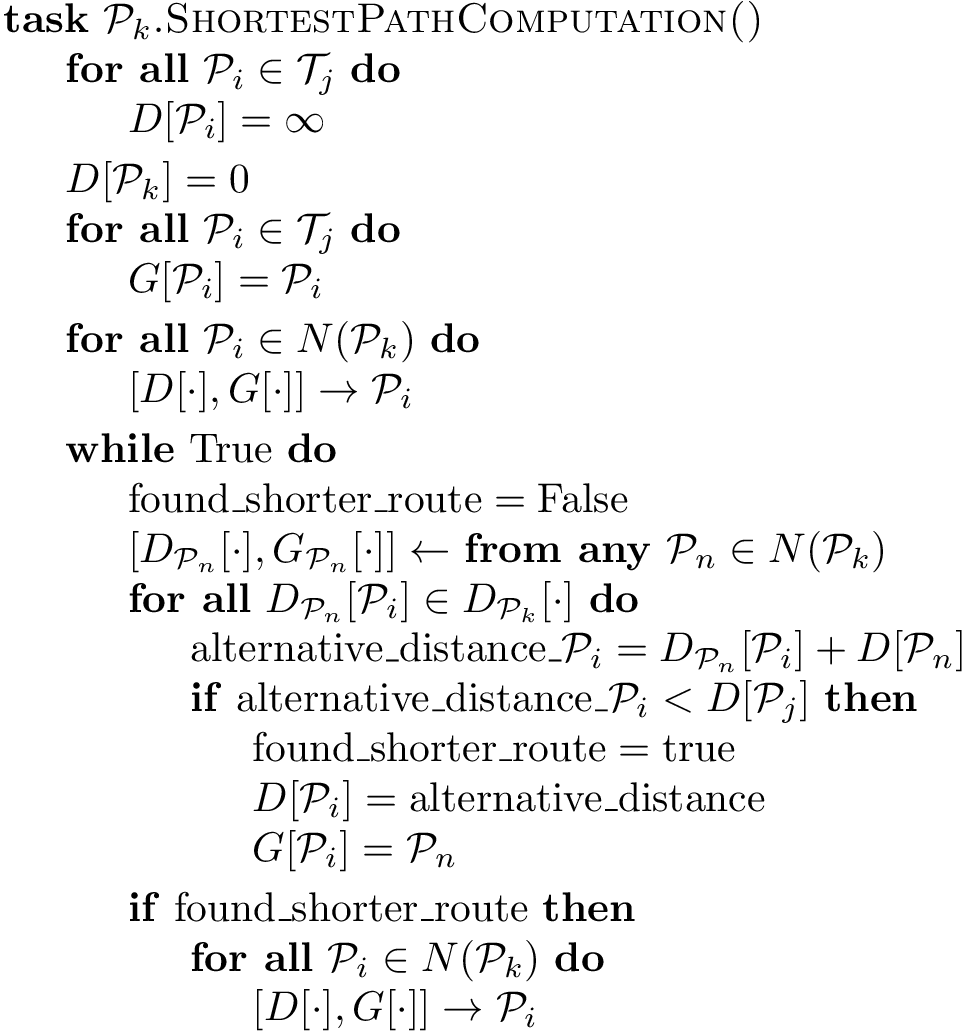
\includegraphics[width=0.35\textwidth]{shortest_path_computation}
  \fig{500}{4cm}{shortest_path_computation}
  \caption{Shortest path computation.\label{fig:shortest_path_computation}}
\end{figure}
The shortest path distances among peers are determined by a variation
of the Bellman-Ford Algorithm~\cite{Bertsekas1987data} (see
Fig.~\ref{fig:shortest_path_computation}), where the cost of the
``links'' between neighbor peers is $1$. Neighbor peers interchange
two vectors $D[\cdot]$ (distance-to-peer) and $G[\cdot]$
(gateway-to-peer) and compute the shortest distances and the (peer)
gateways to (reach) the rest of peers of its team ${\cal T}_j$.

This algorithm is free of routing loops and is not suceptible of the
well known count-to-infinity problem, and therefore always converges
for static teams. These problems do not appear because the routes are 

Each peer ${\cal P}_k$ sends
its vector of distances $D[\forall {\cal P}_i\in T^*({\cal P}_k)]$ and
gateways $G[\forall {\cal P}_i\in T^*({\cal P}_k)]$ to each
neighbor. When this information is received, peers check if shorter
routes can be found to the rest of peers of the reachable team, and if
so, send these vectors again.

The Bellman-Ford algorithm is susceptible of routing loops and the
count-to-infinite problem.


% Hace falta saber desde dónde viene el chunk original (origin peer) y que todos los peers dispongan de los vector-distances de los peers vecinos. Los vector-ditances deben tener tantas entradas como peers existen en el team. Por tanto, cada peer almacena un número de vector-distances igual a su grado de conectividad.


% Supposing that the weight of links between neighbors is 1.
% ¿Cómo sabe un peer que él es el último?
\end{comment}

\begin{comment}
\subsubsection{Generation of the routing tables}
Routing tables has as many entries as peers are in the team. The
routing table of a peer $P_i$ is a dictionary of pairs ($d(P_i, P_j)$,
$P_k$) indexed by the destination peer $P_j$ is a destination peer,
where $d(P_i, P_j)$ is the last measurement of the number of hops (in
peers) between $P_i$ and $P_j$, and $P_k\in N(P_i)$ is the 1-hop peer
that in the shortest-path between $P_i$ and $P_j$. Notice that if
$P_j==P_k$ then $d(P_i, P_j)==1$, which means that $P_i$ and $P_j$ are
directly ``connected''.

When a peer has updated its routing table, it is sent to their
neighbors pyggibacked on a \textsf{chunk} packet. When a peer receives
a routing table, it keeps a copy of it and updates its own routing
table with the new routing information using the Bellman-Ford
Algorithm~\cite{}. The peers have a copy of the routing table of its
neighbors to use it through the chunk routing process (see
Rule~\cite{the_routing_process}.
\end{comment}

